%%
%% CHIIR 2027 short-paper review submission.
%% Maximum four pages for body content; references may extend beyond page four.
%%
%% Commands for TeXCount
%TC:macro \cite [option:text,text]
%TC:macro \citep [option:text,text]
%TC:macro \citet [option:text,text]
%TC:envir table 0 1
%TC:envir table* 0 1
%TC:envir tabular [ignore] word
%TC:envir displaymath 0 word
%TC:envir math 0 word
%TC:envir comment 0 0
%%
\documentclass[sigconf,natbib,anonymous]{acmart}

\usepackage{array}
\usepackage{graphicx}
\graphicspath{{figures/}}
\setkeys{acmart.cls}{balance=false}

\AtBeginDocument{%
  \providecommand\BibTeX{{%
    Bib\TeX}}}

\setcopyright{acmlicensed}
\copyrightyear{2027}
\acmYear{2027}
\acmDOI{}
\acmConference[CHIIR '27]{ACM SIGIR Conference on Human Information Interaction and Retrieval}{March 7--11, 2027}{Berlin, Germany}
\acmISBN{}

\begin{document}
\raggedbottom

\title{A Modular Digitisation Pipeline for Preparing Critical Editions}

\author{Anonymous Author(s)}
\affiliation{%
  \institution{Anonymous Institution}
  \country{Anonymous}
}
\renewcommand{\shortauthors}{Anonymous Author(s)}

\begin{abstract}
Preparing a critical edition of a historical work requires comparing textual variations across editions.
For large works with many editions, the task may become too laborious to tackle manually.
This paper presents a modular digitisation and automation pipeline, illustrated with a working interface, for undertaking such scholarly projects in the humanities.
The pipeline ingests upstream page data containing layout geometry and OCR text, maps display to page images, supports various annotation tasks for page inventory, layout geometry, and text correction, automates logical structure assignment, and shortlists textual changes across editions for examination while retracing the digital text segments to page-image evidence.
This paper describes its implementation in an ongoing critical-edition project of substantial scope: David Hume's \emph{History of England}, with field experts as users, and demonstrates that the modular pipeline approach can help historians get to interpretive work sooner while preserving traceable bibliography to source pages, and that the adaptable conceptual design can generalise to similar document-centric digital humanities projects as well.
\end{abstract}

\begin{CCSXML}
<ccs2012>
 <concept>
  <concept_id>10002951.10003227.10003392</concept_id>
  <concept_desc>Information systems~Digital libraries and archives</concept_desc>
  <concept_significance>500</concept_significance>
 </concept>
 <concept>
  <concept_id>10003120.10003121.10003124</concept_id>
  <concept_desc>Human-centered computing~Interactive systems and tools</concept_desc>
  <concept_significance>300</concept_significance>
 </concept>
 <concept>
  <concept_id>10010405.10010469</concept_id>
  <concept_desc>Applied computing~Arts and humanities</concept_desc>
  <concept_significance>300</concept_significance>
 </concept>
</ccs2012>
\end{CCSXML}

\ccsdesc[500]{Information systems~Digital libraries and archives}
\ccsdesc[300]{Human-centered computing~Interactive systems and tools}
\ccsdesc[300]{Applied computing~Arts and humanities}

% !TEX root = CHIIR-PAPER.tex
\keywords{digitisation, critical editions, digital humanities, text comparison, digital libraries}

\maketitle

\section{Introduction}

Many historical works go through multiple editions of textual changes.
Scholars interested in presenting the work as an evolving entity to capture the nuances of intellectual history, \textit{i.e.} a critical edition, must source and compare the surviving versions and variations of the text, and make interpretations of the editorial changes across time.
This process has traditionally been carried out with manual efforts, which can be time-consuming, error-prone, and difficult to scale.
A historian examining a single revision needs to source rare original copies, find corresponding passages, and visually scan lines of text for variations.
For works that were published multiple times, the task is especially demanding.

One notable example is David Hume's \emph{History of England}: the work circulated in multiple editions and formats, first published in instalments in 1754, 1759, and 1762 in six volumes as \emph{The History of Great Britain}, then rearranged into eight volumes in 1763, followed by multiple editions thereafter.
Hume made thousands of changes at various times in response to historical discourse, culminating in the posthumous 1778 text.
In addition to Hume's editing, which includes substantial changes to the copy text, appendices, footnotes, and other content, the reprinting also resulted in many versions of typesetting formats and artefacts within each edition.
The sheer scale of the materials has previously thwarted any exhaustive manual collation.
When a modern-day reader orders a copy of Hume's \emph{History}, the text available is generally a so-called scholarly or diplomatic edition (such as the Liberty Fund edition~\cite{hume1983liberty}) that is based on the last edition's text, which does not provide the scholarly apparatus for studying textual changes.
While van Holthoon's electronic edition~\cite{vanholthoon2000} attempted to track significant variants, it was never completed, mostly due to the limitation of the traditional manual approach.
Automating the mechanical tasks of this process can save years of repetitive labour and allow historians to focus on their core intellectual work: making interpretations of the textual changes.

This paper presents the conceptual design of a modular digitisation and automation pipeline, implemented as a working interface that helps scholars prepare critical editions.
Upstream computer vision work has enabled layout detection and text recognition, providing page-level XML input mappable to the page images.
The pipeline imports the page data, stores the layout and text as relational records to support annotation tasks of correcting and verifying the digital content and structure, then incorporates digital text processing to compare passages across editions automatically, and presents interfaces for scholars to browse, search through, and zoom in on sites of textual variation for historian review and to perform ``close-reading'' within context on the page, while preserving traceable bibliographical details (\textit{i.e.} on which lines on which pages in which copies of which editions the variations were found) to document the provenance of the interpretive work.
The interface is currently in pilot use, supporting a live editorial project in which intellectual historians are preparing a critical edition of Hume's \emph{History}.

This paper makes three contributions.
First, it describes a modular pipeline that imports upstream page data and produces editable digital layout and text objects that can be interfaced with both machine processing and human annotation.
Second, it presents the workflow for layout and text correction, landmark assignment, text comparison, and scholarly review.
Third, it uses the \emph{History of England} project to show how such a pipeline supports expert historians in a critical-edition workflow, and reports what the comparison procedures emit on one chapter of the ongoing editorial project.

\begin{figure*}[t]
  \centering
  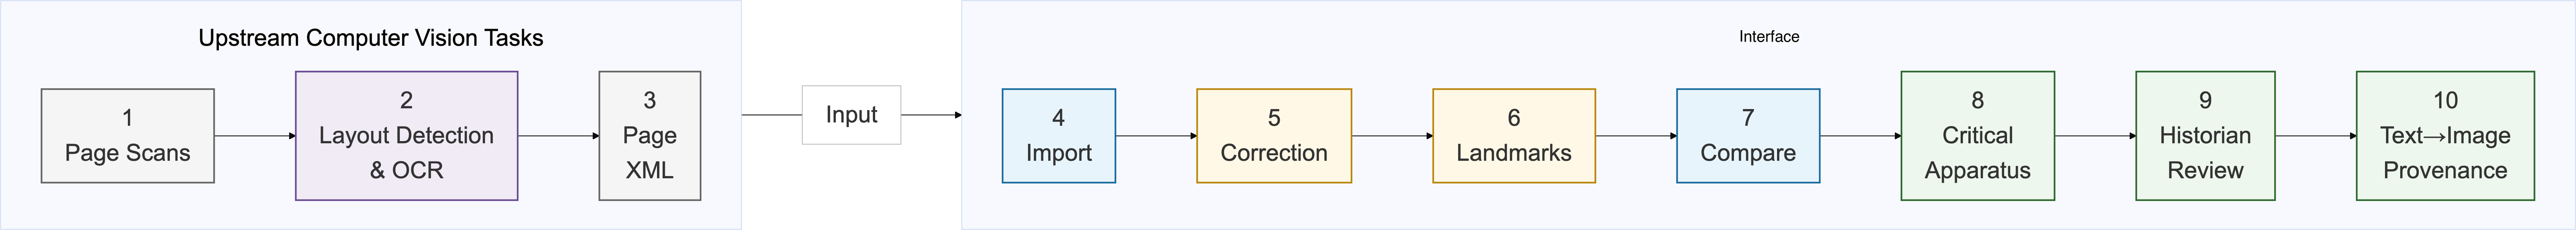
\includegraphics[width=\textwidth]{pipeline-diagram.png}
  \caption{The pipeline imports data from layout detection and OCR, supports geometry and text correction, assigns structure to contents, and provides tools for edition comparison, close reading, and bibliographic tracing.}
  \Description{A workflow diagram with upstream page scans, layout and OCR, and page XML feeding into import, correction, landmarks, comparison, variation sites, historian review, and text-to-image tracing.}
  \label{fig:pipeline}
\end{figure*}

\section{Related Work}

Historians' digital research joins searching and reading with collecting, processing, analysing, and writing, and a scholarly question needs an access point in the document itself~\cite{korkeamaki2019interacting,kumpulainen2020historical}.
For a critical edition, that access point is a site of variation which can still be checked against the printed page.
Transkribus makes recognition models replaceable inside a transcription environment~\cite{kahle2017transkribus}, but it does not carry a corrected corpus through multi-edition comparison and page-image provenance.
CollateX separates tokenisation, alignment, analysis, and visualisation while leaving interpretation to scholars~\cite{haentjensdekker2014collation}.
The Versioning Machine presents encoded versions alongside images~\cite{schreibman2003versioning}, and Juxta, LERA, and Variance Viewer offer further workflows for encoded texts~\cite{roeder2019collation}.
Text-reuse methods can find shared passages across large collections~\cite{smith2015reprinted}.
The comparison here begins after corresponding paragraphs have been linked, and then separates sentences with high overlap from larger divergences.
Visibility, correction, and user control remain necessary once a computation produces a reading that a historian may rely on~\cite{amershi2019guidelines}.

\section{Method}

The conceptual design of the pipeline, as shown in Figure~\ref{fig:pipeline}, treats document digitisation as a sequence of components rather than as a one-size-fits-all processing job that converts page images to OCR text.
Upstream components start with page images, often from sources of uneven quality, and perform image pre-processing, layout detection, line detection, and optical character recognition (OCR) to produce one XML file per page, mapped to the page image.
The pipeline imports those page images and XML-derived data, and persists pages, layout regions, line geometry, and the text of each line as records that later annotation and comparison can use.
Imported values remain distinguishable from later attributed edits.
A string shown in comparison can therefore be followed through its logical unit and constituent lines to the regions from which it was transcribed.

\textbf{Data correction.}
Page images in the present project come from library photographs, through the Internet Archive, and from digitised microfilm.
After import, annotators reconcile page order, printed numbering, duplicate pages, and skipped scans, including a corrected number where the printed number is wrong.
In the geometry view, numbered boxes are overlaid on the facsimile.
The annotator selects a region or line, adjusts a misplaced boundary, drops an artefact, or adds a missing line, including the double-height boxes that layout detection sometimes produces.
In the copytext view, selecting a line connects its OCR string with a cropped image of that line, and a correction is saved without discarding the imported value.
A volume can contain hundreds of missing or misread lines, and those have to be corrected before a textual difference can be treated as a property of the edition rather than of the digitisation.

\textbf{Structural alignment.}
For editions to be comparable, landmarks must be assigned so that lines are nested in chapters, sections, and paragraphs.
Each unit is an abstract entity within the work that manifests as different blocks of lines on different pages, depending on the edition and its typesetting.
The corresponding block in each edition is aligned to the 1778 text, which is the lemma, so that historians can compare the same passage across editions (Figure~\ref{fig:align}).
An automated first pass uses regularities of the print: a paragraph typically starts on a new line with a capitalised opening, sections are preceded by a vertical gap and sometimes by a heading, and chapters start on a new page.
Annotators then correct the node boundaries.
Where one edition splits or merges a paragraph, a positional marker identifies a pseudo-paragraph, so that part of one paragraph can correspond to a whole paragraph elsewhere.
Comparison does not rediscover these links.
If the link is missing, that edition is absent from the comparison.

\textbf{Text comparison.}
Lines within an aligned paragraph are joined into running text.
A hyphen that exists only to break a word at the end of a line is dropped, while a hyphen that belongs to the word is kept.
The character-to-line mapping is retained.
Two procedures then use that reading text, and they answer different questions.
Sentence splitting belongs only to the pairwise procedure.

The pairwise interface takes two editions and separates stretches that still have high overlap from stretches that have diverged substantially (Figure~\ref{fig:diff}).
Each paragraph is divided into sentence-like blocks, and a long sentence that contains several shorter ones is divided at those seams.
Blocks with high overlap are compared word by word, with letter alignment inside a substitution, so spelling, punctuation, and long~s remain visible inside the word.
Sentences that fail the overlap test stay whole, as additions, omissions, or unequal blocks.
A word alignment forced onto a rewritten sentence would paint nearly every word as a change and hide that the sentence is no longer the same unit.

The multi-edition interface takes one lemma paragraph and every edition aligned to it, and records where the paragraph varies and what each edition reads there (Figure~\ref{fig:candidate}).
Each edition is aligned independently to the lemma.
Insertions, omissions, and replacements become intervals on the lemma.
A replacement that differs only by long~s does not open a site; other spelling changes, wording changes, and differences of case are kept.
Intervals only a few words apart are grouped into one site, except across a clause or sentence break, and words that every edition shares at the edges are trimmed into locating context, about two words on either side.
For every site the interface stores the reading of every aligned edition, including an edition that agrees with the lemma and an edition that has nothing between the surrounding words.
The output is a candidate list for historian review, not a finished scholarly or TEI apparatus.
The historian decides whether a difference is typographical, accidental, or historically meaningful.

\textbf{Traceability.}
Both procedures display the spans already computed.
They do not recompute the comparison in order to paint the page.
Each digital segment is traced to bounding boxes on the page image of the relevant edition, so the same reading can be checked in its printed line and in the surrounding context of the page.

\begin{figure}[t]
  \centering
  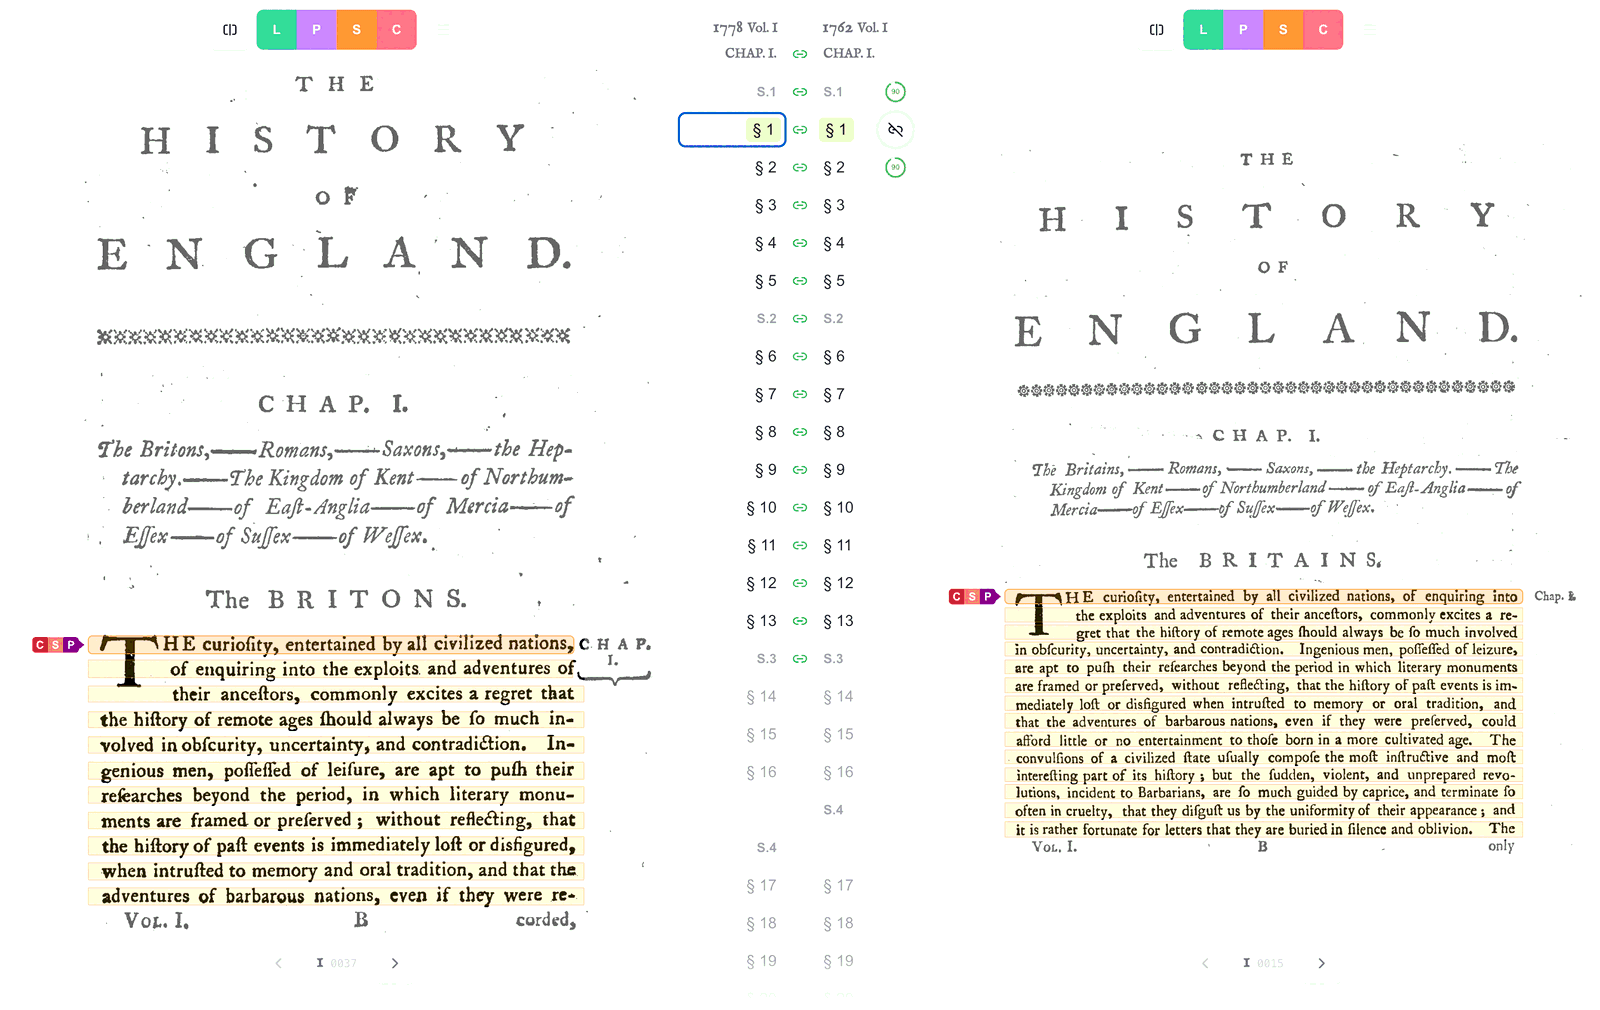
\includegraphics[width=\columnwidth]{align-paragraphs.png}
  \caption{Paragraph alignment links Chapter~I across the 1778 and 1762 editions. Central controls record the correspondence that later comparison requires.}
  \Description{Two facsimile pages appear side by side with a central column of paragraph-link controls. Corresponding openings of Chapter~I are highlighted on each page.}
  \label{fig:align}
\end{figure}

\begin{figure}[t]
  \centering
  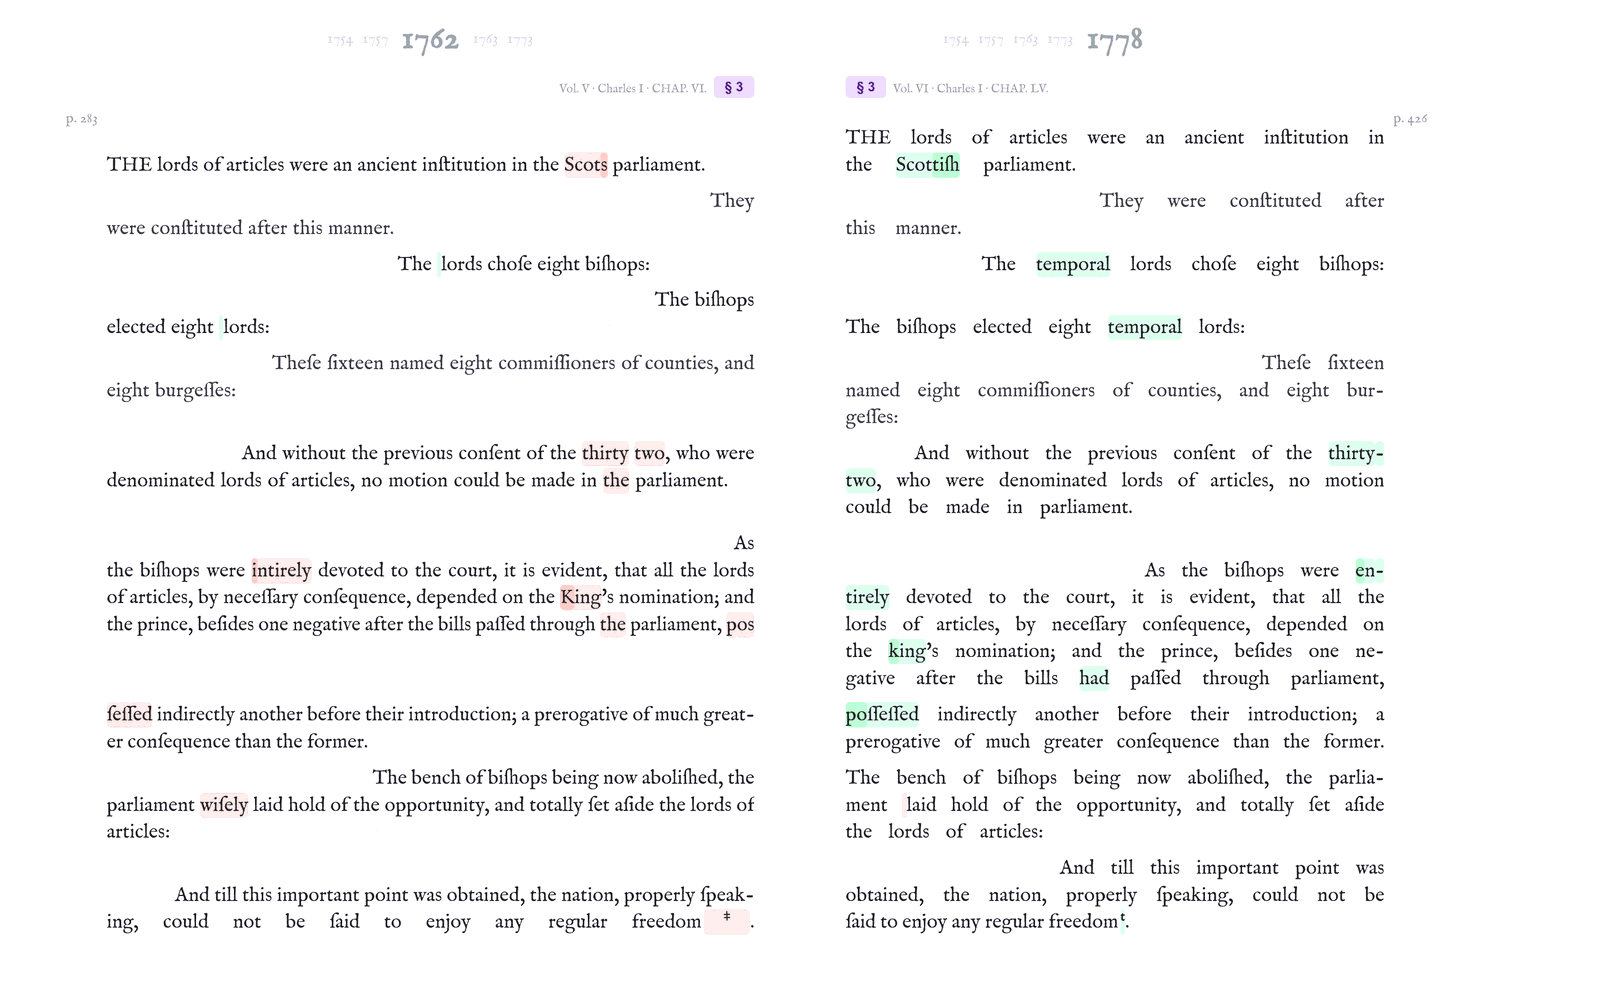
\includegraphics[width=\columnwidth]{diff-sentences.png}
  \caption{Pairwise comparison of a Charles~I passage from 1762 and 1778. High-overlap sentences receive local highlighting, while larger divergences remain whole blocks.}
  \Description{Two columns of edition text show highlighted word and character differences, with edition years and page references above the columns.}
  \label{fig:diff}
\end{figure}

\begin{figure*}[t]
  \centering
  \setlength{\abovecaptionskip}{2pt}
  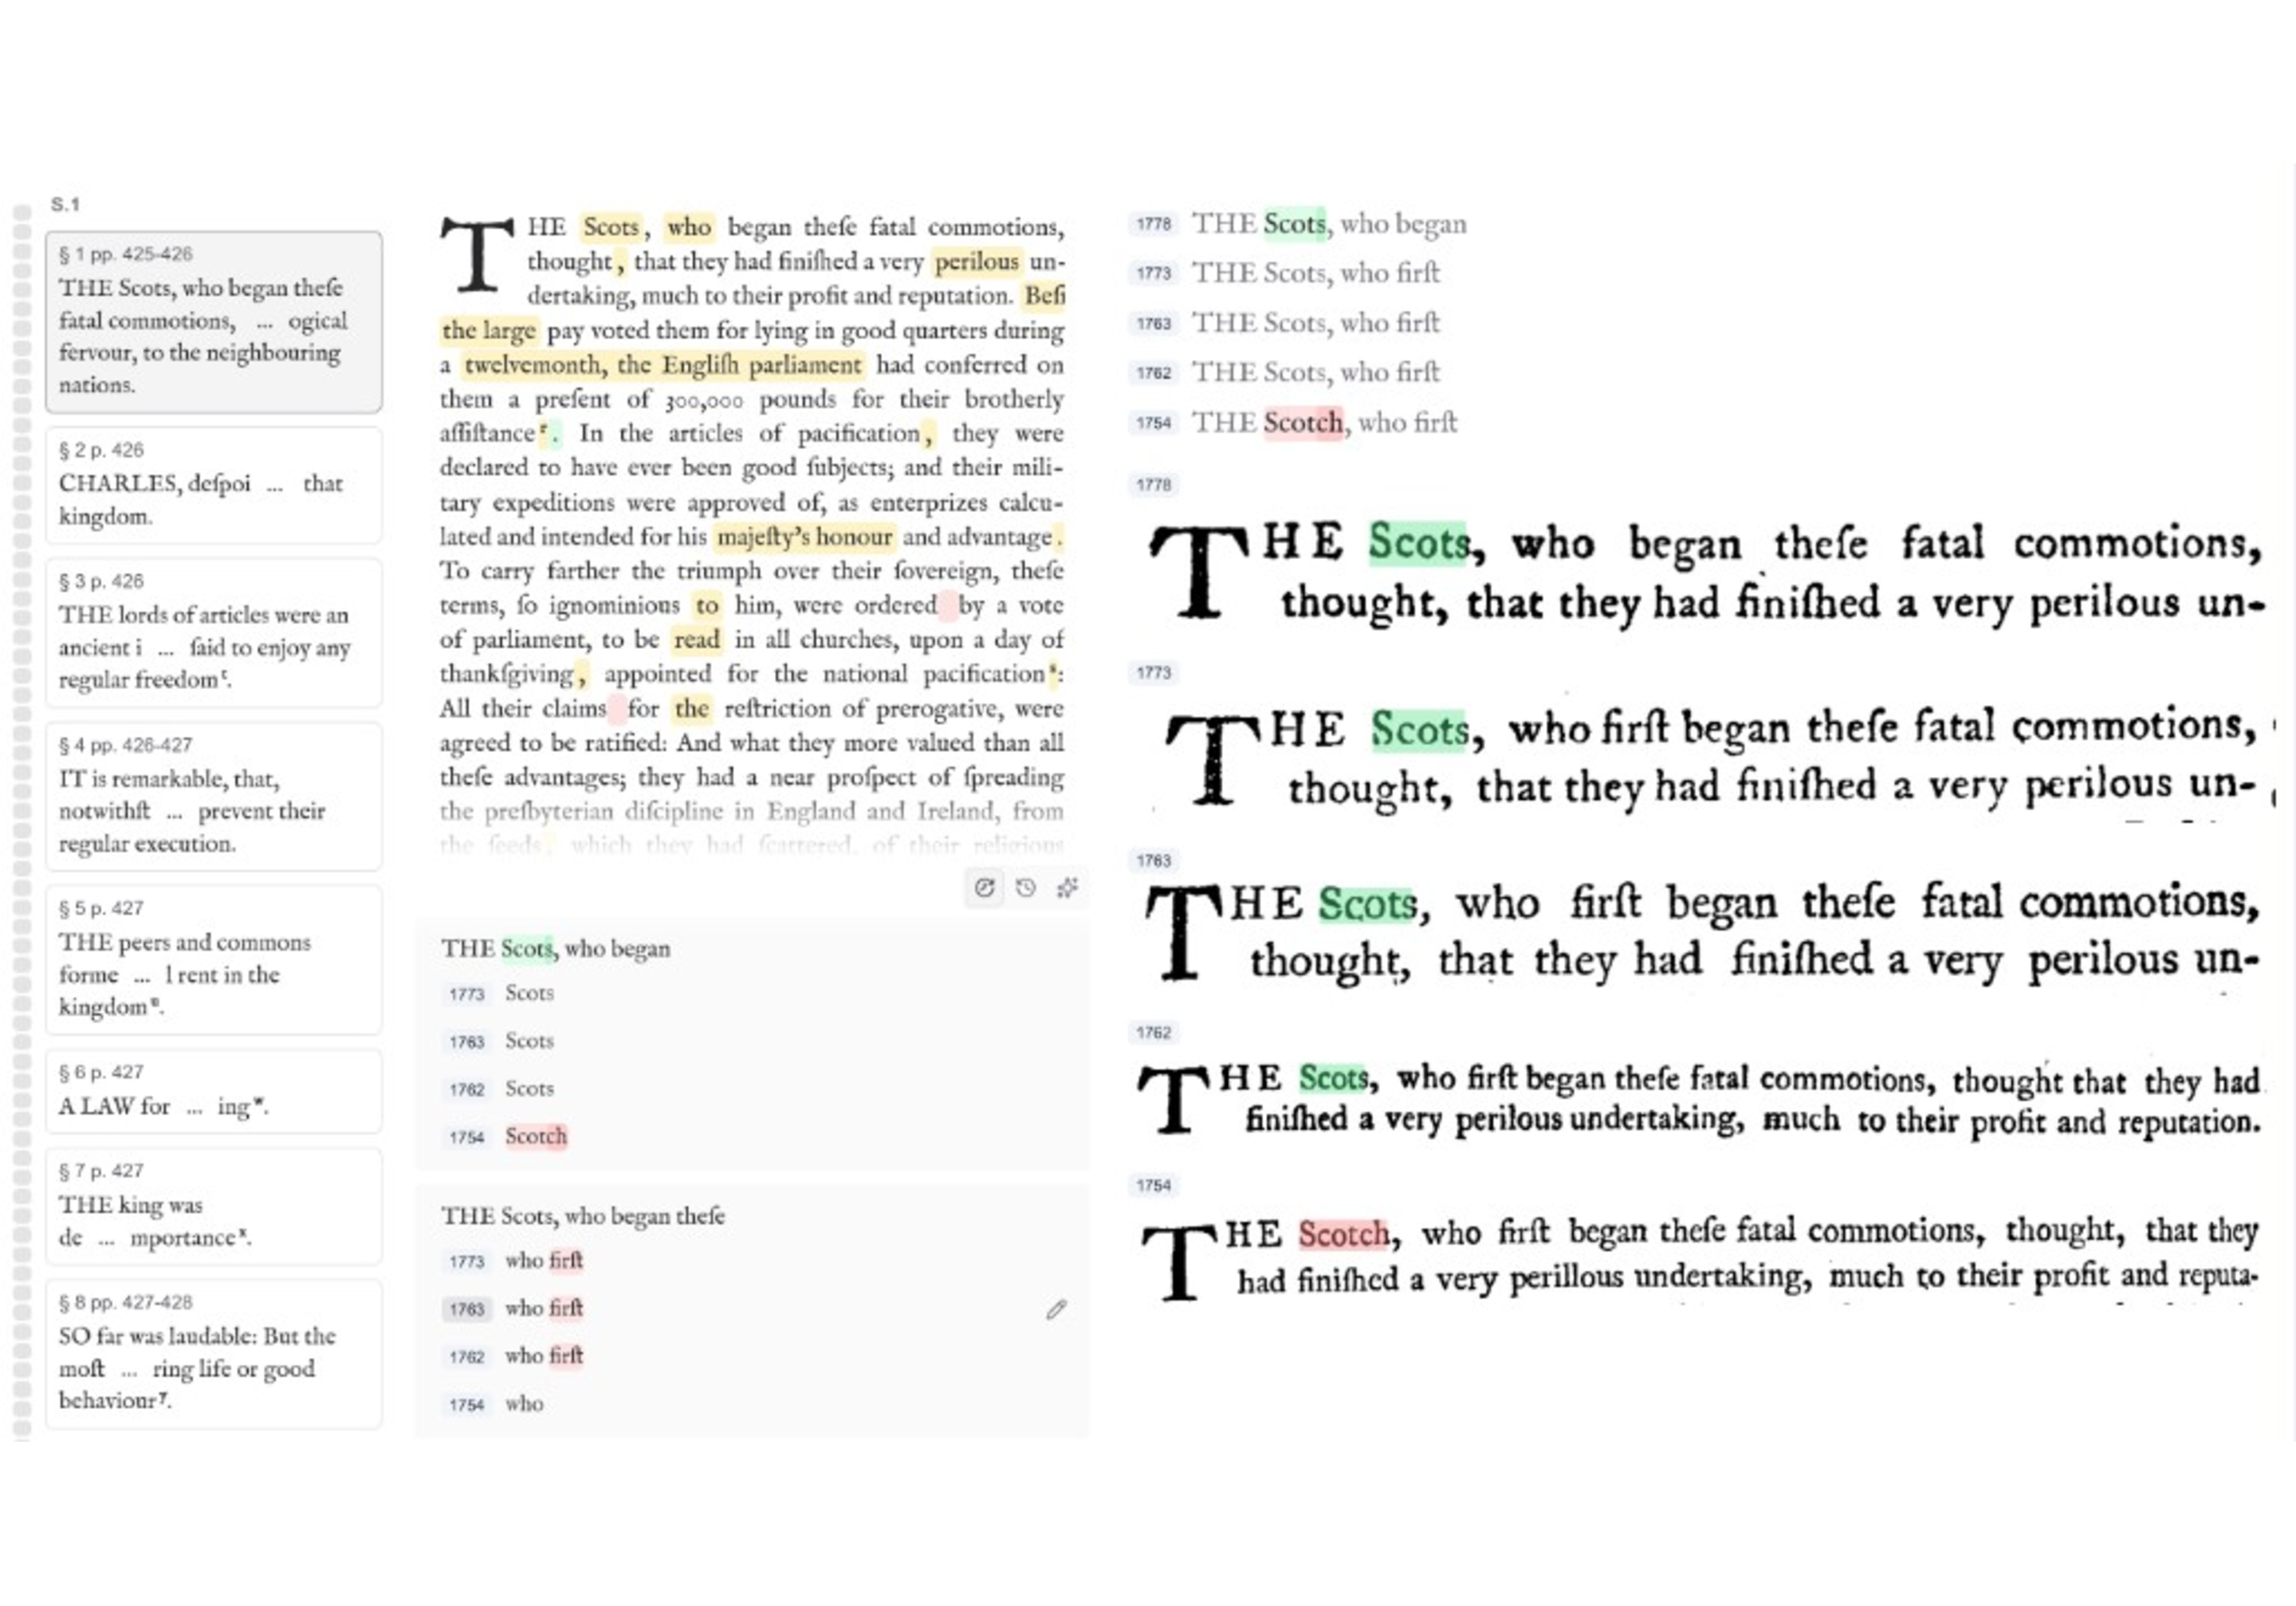
\includegraphics[width=\textwidth]{candidate-facsimile.png}
  \caption{Candidate readings with edition-specific facsimile snippets across 1778--1754.}
  \Description{A paragraph navigator appears on the left, a selected passage with marked candidate readings in the centre, and stacked cropped facsimile lines labelled by edition year on the right.}
  \label{fig:candidate}
\end{figure*}

\section{Evaluation}

For illustration, this section show-cases the results of an example run of the text processing over Chapter~LV concerning the reign of Charles I. Five editions have aligned structural nodes within the corpus: 1754, 1762, 1763, 1773, and 1778 (lemma).

\begin{table}[t]
  \caption{Chapter scale for the five aligned editions. The 1778 text is the lemma.}
  \label{tab:chapter}
  \small
  \begin{tabular}{@{}>{\raggedright\arraybackslash}p{0.28\columnwidth}rrr@{}}
    \toprule
    Edition & Paragraphs & Sentences & Words \\
    \midrule
    1754 & 113 & 717 & 20,424 \\
    1762 & 112 & 708 & 20,376 \\
    1763 & 112 & 701 & 20,159 \\
    1773 & 113 & 699 & 20,210 \\
    1778 & 110 & 673 & 19,676 \\
    \bottomrule
  \end{tabular}
\end{table}

\begin{table}[t]
  \caption{High-overlap and large-divergence words in the 1754--1778 comparison. Percentages use each edition's chapter word count.}
  \label{tab:pairwise}
  \small
  \begin{tabular}{@{}>{\raggedright\arraybackslash}p{0.22\columnwidth}rr@{}}
    \toprule
    Edition & High overlaps & Large divergence \\
    \midrule
    1754 & 19,278 (94.4\%) & 1,147 (5.6\%) \\
    1778 & 19,337 (98.3\%) & 339 (1.7\%) \\
    \bottomrule
  \end{tabular}
\end{table}

\textbf{Pairwise comparison.}
The 1754--1778 comparison contains 109 paragraph pairs.
One 1778 paragraph and four 1754 paragraphs have no counterpart.
The procedure produced 679 sentence rows with high overlap, eight sentences only in 1778, 43 only in 1754, and two unequal block pairs.
Within the high-overlap rows it reported 590 words only in 1754, 568 words only in 1778, and 1,055 substitutions: 22 differing only by long~s, 183 only by capitals, and 850 by other wording or spelling.
The 1754 counts in Table~\ref{tab:pairwise} sum to 20,425, one above the 20,424 words of the chapter, because dividing a fused sentence restores a space that the joined paragraph did not count as a word.

\begin{table}[t]
  \caption{Transformation of lemma--edition differences into candidate sites across 1754, 1762, 1763, 1773, and the 1778 lemma.}
  \label{tab:apparatus}
  \small
  \begin{tabular}{@{}>{\raggedright\arraybackslash}p{0.67\columnwidth}r@{}}
    \toprule
    Measure & Output \\
    \midrule
    Hard lemma--edition change pairs & 6,741 \\
    Long-s-only replacements excluded & 165 \\
    Grouped candidate sites & 2,398 \\
    Modification sites & 1,364 (56.9\%) \\
    Deletion in lemma & 791 (33.0\%) \\
    Lemma wording absent as a block & 243 (10.1\%) \\
    Median sites per lemma paragraph & 14 \\
    Lemma words inside site cores & 3,127/19,676 (15.9\%) \\
    \bottomrule
  \end{tabular}
\end{table}

\textbf{Sites of variation.}
Every lemma paragraph has at least one linked edition.
Alignment against the lemma produced 6,741 hard change pairs, and a further 165 replacements were only long~s and were set aside.
Grouping nearby differences, without crossing a clause break, turned those 6,741 pairs into 2,398 sites (Table~\ref{tab:apparatus}).
The median is 14 sites per paragraph, and 3,127 of the lemma's 19,676 words fall inside a site core.
At the opening site the lemma reads \emph{Scots}; 1754 reads \emph{Scotch}, while 1762, 1763, and 1773 agree with 1778.
That cell shows the form of an entry.
It is not a summary of Hume's revision history.

One of the paragraph links joins passages that are not the same length.
The 1778 paragraph beginning ``The pulpits likewise were called in aid'' is 62 words, but the paragraph aligned to it is 292 words in 1754 and 252 words in 1762 and 1763.
Only the 1773 paragraph matches the lemma, at 62 words.
The comparison does not split a paragraph it has been given, so the extra wording is recorded as places where the 1778 text has nothing between the surrounding words.
That one link produces 610 sites, 604 of them deletions in the lemma, and those 604 are most of the 791 deletions in the chapter.
Set that paragraph aside and the mean is 16.4 sites rather than 21.8, and the longest of the rest has 68 sites rather than 610.
Pairwise comparison leaves the extra sentences whole, which is why Table~\ref{tab:pairwise} counts 1,147 words of large divergence in 1754 rather than hundreds of one-word sites.
A further 725 sites have a lemma core that matches every linked reading once long~s is set aside: 644 are deletions in the lemma, including the 604 from this paragraph, and 81 are cores tightened until nothing differed.
A site in the list is therefore not, by itself, a disagreement the editions display.

\section{Discussion}

The Hume corpus is distinctive in its size and publication history, but the workflow is a common one: collect page images, process them into machine-readable data, correct and structure the text, compare differences, and link each segment back to the page.
The same pipeline can be adapted for another document-based project once corresponding passages can be aligned and the printed page remains available for checking.
The chapter shows that the two grains are not interchangeable: the pairwise view keeps unmatched sentences whole, while the apparatus records that extra wording as hundreds of deletions in the lemma rather than as whole blocks.

\textbf{Limitations.}
Image quality, layout detection, and OCR performance affect the text that annotators must correct, and correction across the wider project remains uneven.
The evaluation uses one chapter and its existing paragraph links.
It does not measure precision or recall against a scholar's collation.
Which variations are historically significant remains for the historian to decide, facsimile rights constrain redistribution, and the same rules have not been tested on other typographies or any other editorial conventions.

\section{Conclusion}

The pipeline carries page images through correction, alignment, and textual comparison while keeping each segment traceable to the printed line.
Shortlisting sites of variation, and leaving the facsimile available for checking, allows humanities scholars to devote more of their time and effort to interpretive work across the editions.

%% Acknowledgements are omitted from the anonymous review version.
\begingroup
\setlength{\bibsep}{0pt plus 0.3\baselineskip}
\bibliographystyle{ACM-Reference-Format}
\bibliography{references}
\endgroup

\end{document}
